\chapter{Termo de Abertura do projeto}

\section{EAP}
\begin{figure}[!htb]
    \center{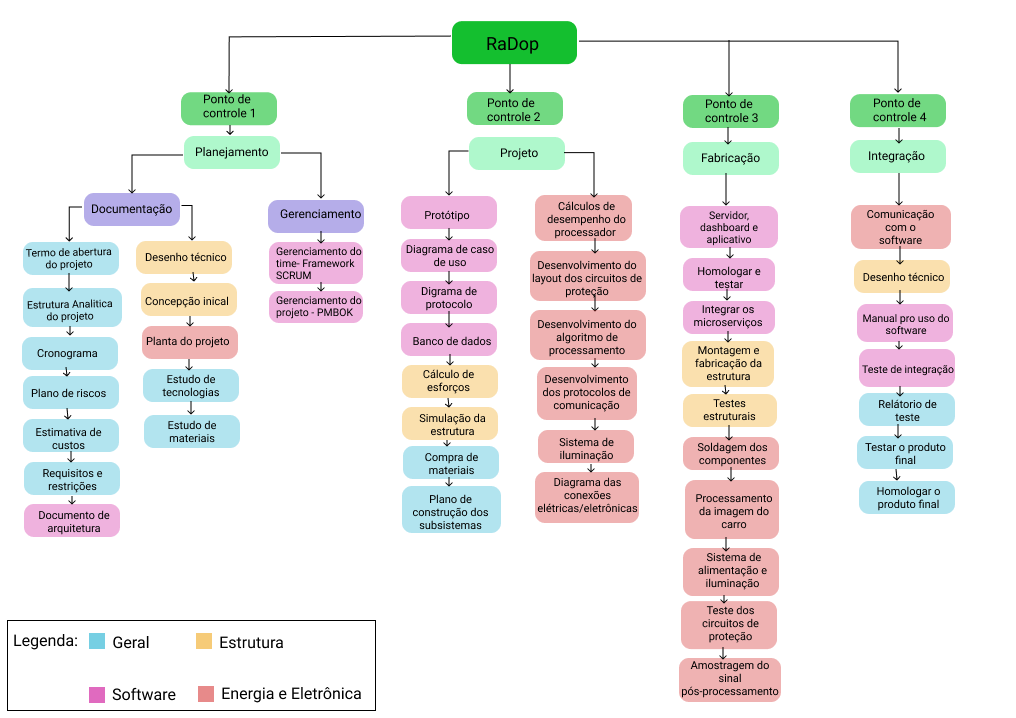
\includegraphics[width=\textwidth]{eap.eps}}
    \caption{\label{fig:eap} EAP do projeto}
\end{figure}
\section{Lista É/Não é}
\subsection{É}
\subsection{Não é}
\section{Requisitos}
\subsection{Eletrônica}
\subsection{Energia}
\begin{itemize}
	\item O sistema deve conter painéis fotovoltaicos que promoverão a fonte de alimentação para todos os componentes do sistema;
	\item O sistema deve garantir o máximo aproveitamento energético;
	\item O sistema deve conter circuitos de controle de tensão e corrente;
	\item O sistema deve conter circuitos de controle de tensão e corrente;
	\item O sistema deve garantir o funcionamento seguro e contínuo do Radar;
	\item O sistema deve conter um circuito de iluminação para servir de alerta aos motoristas;
	\end{itemize}

	\vspace*{\fill}
    \pagebreak
    
\subsection{Estrutura}
\subsection{Software}
\section{\emph{Stakeholders}}
\section{Recurso humanos}
\section{Cronograma de atividades}



\section{Milestones Identificados}
\section{Estimativa de custos}
\subsection{Orçamento preliminar}
\begin{table}[h]
\centering
\caption{Estimativa de custos de eletrônica}
\label{custos_eletronica}
\begin{tabular}{|c|c|c|c|c|}
\hline
\multicolumn{5}{|c|}{Eletrônica} \\ \hline
Quantidade & Material & Valor Unitário & Total & Fornecedor \\ \hline
02 & BeagleBone & R\$ 320,00 & R\$ 640,00 & Mercado Livre \\ \hline
02 & Módulos GSM & R\$ 99,90 & R\$ 199,90 & TDTEC \\ \hline
02 & Módulos RF & R\$ 32,90 & R\$ 65,80 & HU Infinito \\ \hline
10 & \begin{tabular}[c]{@{}c@{}}Componentes para Placa\\  de Circuito Impresso\end{tabular} & R\$ 40,00 & R\$ 400,00 & HU Infinito \\ \hline
02 & Antena painel & R\$ 108,80 & R\$ 217,60 & Emprestado \\ \hline
02 & BladeRF NUAND & R\$ 3.000,00 & R\$ 6.000,00 & Emprestado \\ \hline
02 & Circulador & R\$ 150,00 & R\$ 300,00 & Emprestado \\ \hline
02 & Câmera & R\$ 1.000,00 & R\$ 2.000,00 & Em análise \\ \hline
X & Componentes diversos & R\$ 50,00 & R\$ 50,00 & HU Infinito \\ \hline
Total & - - & - - & R\$ 9873,30 & - - \\ \hline
\end{tabular}
\end{table}
\section{Viabilidades financeira}
\section{Levantamento de riscos}
<<<<<<< HEAD
=======

\begin{comment}
\begin{description}
	\item [Pré-textuais] \

	\begin{itemize}
		\item Capa
		\item Folha de rosto
		\item \textit{Dedicatória}
		\item \textit{Agradecimentos}
		\item \textit{Epígrafe}
		\item Resumo
		\item Abstract
		\item Lista de figuras
		\item Lista de tabelas
		\item Lista de símbolos e
		\item Sumário
	\end{itemize}

	\item [Textuais] \

	\begin{itemize}
		\item \textbf{\textit{Introdução}}
		\item \textbf{\textit{Desenvolvimento}}
		\item \textbf{\textit{Conclusões}}
	\end{itemize}

	\item [Pós-Textuais] \
	
	\begin{itemize}
		\item Referências bibliográficas
		\item \textit{Bibliografia}
		\item Anexos
		\item Contracapa
	\end{itemize}
\end{description}

\end{comment}

>>>>>>> 4ef4c5a9d179b0ced8d6ff52122a2aacd641c19d
